\documentclass{article}
\usepackage[a4paper, total={6in, 8in}]{geometry}
\usepackage{amsmath} 
\usepackage{graphicx}
\graphicspath{ {images/} }

\title{Analyzing the choice of transportation}
\author{Elie Daher}

\begin{document}
\pagenumbering{gobble}
\maketitle
\abstract This document contains the problem of analysing the choice of transportation. This problem is from the chapter UTA Methods of the Book: Multiple Criteria Decision Analysis. This document was made during my internship at LAMSADE in the summer of 2017.\\

A DM wants to analyse the choice of transportation. The DM is interstered in the following criteria 
\begin{enumerate}
\item price
\item time (min)
\item comfort (possibility to have a seat)
\end{enumerate}\leavevmode

The evaluation of the previous criteria:
\begin{center}
\begin{tabular}{ |c|c|c|c|c| } 
\hline
Means of transportation & Price & Time & Comfort & Ranking of the DM \\
\hline
RER & 3 & 10 & + & 1 \\
METRO (1) & 4 & 20 & ++ & 2 \\
METRO (2) & 2 & 20 & 0 & 2 \\
BUS & 6 & 40 & 0 & 3 \\
TAXI & 30 & 30 & +++ & 4 \\
\hline
\end{tabular}
\end{center}

DM's preferences: $ RER \succ  Metro1 \approx Metro2  \succ  Bus \succ  Taxi$\\

\newpage

\section{Scale for each criteria}
For each criteria, the interval $[g_i^{*}, g_{i*}]$ is cut into $(\alpha _i -1)$ equal intervals. So in this case we have: 
\begin{itemize}
\item Price  $\quad \rightarrow \quad [30, 16, 2]$
\item Time  $\quad \rightarrow \quad [40, 30, 20, 10]$
\item Comfort  $\quad \rightarrow \quad [0, +, ++, +++]$
\end{itemize}

\section{Marginal value by linear interpolation}
The marginal value is calculated by a linear interpolation. In this case we have: 
\begin{itemize}
\item $v[g(RER)]= 0.07  v_1 (16) + 0.93 v_1(2) + v_2(10) + v_3(+)$
\item $v[g(METRO1)]= 0.14 v_1 (16) + 0.86 v_1(2) + v_2(20) + v_3(++)$
\item $v[g(METRO2)]= v_1 (2) + v_2(20) + v_3(0) =  v_1 (2) + v_2(20) $
\item $v[g(BUS)]= 0.29  v_1 (16) + 0.71 v_1(2) + v_2(40) + v_3(0) = 0.29 v_1 (16) + 0.71 v_1(2)$
\item $v[g(TAXI)]= v_1 (30) + v_2(30) + v_3(+++) = v_2(30) + v_3(+++)$
\end{itemize}

\section{Replace $v_i$ with $w_{ij} $}
\begin{itemize}
\item $v[g(RER)]= w_{11} + 0.93 w_{12} + w_{21} + w_{22} + w{23} + w_{31}$
\item $v[g(METRO1)]=w_{11} + 0.86 w_{12} + w_{21} + w_{22} + w_{31} + w_{32}$
\item $v[g(METRO2)]= w_{11} + w_{12} + w_{21} + w_{22} $
\item $v[g(BUS)]= w_{11} + 0.71 w_{12}$
\item $v[g(TAXI)]= w_{21} + w_{31} + w_{32} + w_{33}$
\end{itemize}

\section{Difference between each pair of consecutive actions}
\begin{itemize}
\item $\Delta (RER, METRO1) = 0.07 w_{12} + w_{23} - w_{32} + \sigma_{RER} - \sigma_{METRO1} \geq \delta$
\item $\Delta (METRO1, METRO2) = -0.14 w_{12} + w_{31} + w_{32} + \sigma_{METRO1}- \sigma_{METRO2} = 0$
\item $\Delta (METRO2, BUS) = 0.29 w_{12} + w_{21} + w_{22} + \sigma_{METRO2} - \sigma_{BUS} \geq \delta$
\item $\Delta (BUS, TAXI) = w_{11} + 0.71w_{12} - w_{21} - w_{31} - w_{32} - w_{33} + \sigma_{BUS} - \sigma_{TAXI} \geq \delta$
\end{itemize}

\section{Linear Program}
Main objectif: $[min]F = \sum_{a \in A_R} \sigma(a) $ \\
subject to : 
$$\Delta (RER, METRO1)\geq \delta$$
$$\Delta (METRO1, METRO2) = 0$$
$$\Delta (METRO2, BUS)\geq \delta$$
$$\Delta (BUS, TAXI) \geq \delta$$
$$\sum_{i=1}^{n} u_i(g_{i}^{*}) = 1$$
	
With $[min]F = \sum_{a \in A_R} \sigma(a) $ as the main objectif, we have the following linear program to solve: 
 
\begin{center}
\begin{tabular}{ |c|c|c|c|c|c|c|c|c|c| } 
\hline Desc & $w_{11}$ & $w_{12}$ & $w_{21}$ & $w_{22}$  & $w_{23}$ & $w_{31}$ & $w_{32}$ & $w_{33}$ & Result  \\ \hline
$\Delta (RER, METRO1)\geq \delta$     & 0 & 0.07  & 0  & 0 & 1 & 0  & -1 & 0 & $\geq \delta$\\
$\Delta (METRO1, METRO2) = 0$         & 0 & -0.14 & 0  & 0 & 0 & 1  & 1  & 0 & $= 0$\\
$\Delta (METRO2, BUS)\geq \delta$     & 0 & 0.29  & 1  & 1 & 0 & 0  & 0   & 0 & $\geq \delta$\\
$\Delta (BUS, TAXI) \geq \delta$          & 1 & 0.71  & -1 & 0 & 0 & -1 & -1 & -1 & $\geq \delta$\\
$\sum_{i=1}^{n} u_i(g_{i}^{*}) = 1$ & 1 & 1       & 1   & 1 & 1 & 1  & 1  & 1 & $= 1$ \\
\hline
\end{tabular}
\end{center}

So by using the com.google.ortools library, we can solve the Linear Program above with $\sigma = 0.05$. This Linear Program solution is coded in Java class ChoiceTransportation.
\begin{center}
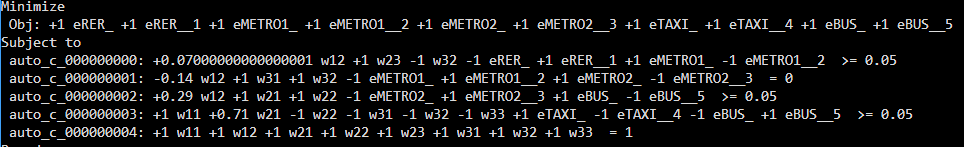
\includegraphics{example_choicetransportation_lp}
\end{center}

An optimal solution has been found of the LP with $\sigma = 0.05$. The objective was accomplished with $[min]F = \sum_{a \in A_R} \sigma(a) = 0$ and $w_{11} = 0.5$, $w_{22} = 0.05$, $w_{23} = 0.05$, $w_{33}=0.4$. 

\begin{center}
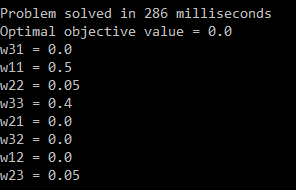
\includegraphics{example_choicetransportation_solution}
\end{center}

\end{document}